\section{Feedback in state space. The Linear Quadratic Regulator}
\label{chap:control_sec:lqrDesign}
The quadratic optimal control method is one of the control methods applied in state space systems and it provides a systematic way of computing the state feedback control gain matrix \cite{Ogata}.
Given the state space system equation
\begin{equation}
\mathbf{\dot{x}} = \mathbf{A}\textbf{x} + \mathbf{B}\mathbf{u}
\end{equation}
the LQR determines the matrix $\mathbf{K}$ of the optimal control vector
\begin{equation}
\mathbf{u}(t) = -\mathbf{Kx}(t)
\label{eq:control}
\end{equation}
so as to minimize the performance index
\begin{equation}
J = \int_{0}^{\infty}(\mathbf{x}^{T}\mathbf{Qx}+\mathbf{u}^{T}\mathbf{Ru}) dt
\end{equation}

where $\mathbf{Q}$ is a positive-definite (or positive-semidefinite) Hermitian or real symmetric matrix and $\mathbf{R}$ is a positive-definite Hermitian or real symmetric matrix. Note that matrices $\mathbf{Q}$ and $\mathbf{R}$ determine the relative importance of the error and the expenditure of the energy of the control signals.
The linear control law given by equation \eqref{eq:control} is the optimal control law. Therefore, if the unknown elements of the matrix $\mathbf{K}$ are determined so as to minimize the performance index, then $\mathbf{u}(t) = -\mathbf{Kx}(t)$  is optimal for any initial state $x(0)$. 

The optimum $K$ matrix is obtained from equations \ref{eq:Kcont} and \ref{eq:Kdisc}.
\begin{equation}
K = R^{-1}B^{T}P \quad (continuous \quad case)
\label{eq:Kcont}
\end{equation}
\begin{equation}
K = (R + B^{T}PB)^{-1}B^{T}PA \quad (discrete \quad case)
\label{eq:Kdisc}
\end{equation}

where $P$ is a positive-definite Hermitian or real symmetric matrix obtained from the algebraic Ricatti Equation:
\begin{equation}
P \rightarrow A^{T}P+PA-PBR^{-1}B^{T}P+Q = 0 \quad (continuous \quad case)
\end{equation}
\begin{equation}
P \rightarrow A^{T}PA+P-A^{T}PB(R+B^{T}PB)^{-1}B^{T}PA+Q = 0 \quad (discrete \quad case)
\end{equation}


In order to obtain the controller design for further simulations and experiments, the following mechanical parameters of the inverted pendulum (corresponding to Rh-2 humanoid robot) were taken: $m$ = 62.589 kg, $l$=0.8927 m, $k$=200. The high stiffness value is due to the rigidity of the pendulum (the leg in this case). If it has a high stiffness, the pendulum will behave as a so rigid link, but if it is lower, the pendulum will be considered as a flexible link and will react in a slower way.

For the optimum response of the control system, we take $Q = C^{T}C = \begin{bmatrix}
0.9487 & 0\\
0 & 0
\end{bmatrix}$ and $R = \mathbf{Q}$. 
%%% AÑADIR SOLO SI SE PRUEBA QUE ES MAS RAPIDO %%%%
%But for a faster response of the control, we take $Q = C^{T}C = \begin{bmatrix}
%1000 & 0\\
%0 & 0
%\end{bmatrix}$.  
After the LQR controller was designed, the following parameters were obtained using a sample time $T = 0.03$ s.

\begin{align}
\mathbf{A} = 
	\begin{bmatrix}
		1.003 & 0.03003 \\
		0.2096 & 1.003
	\end{bmatrix}; & \quad
\mathbf{B} = 
	\begin{bmatrix}
		0.0004502\\
		0.03003
	\end{bmatrix}; \nonumber \\
\mathbf{C} = 
	\begin{bmatrix}
		-1.3060 & 0
	\end{bmatrix}; & \quad
D = 0.3257;
\end{align}
\begin{equation}
\mathbf{K} = 
	\begin{bmatrix}
		13.5366 & 5.1035
	\end{bmatrix}
\end{equation}

The block diagram showing the optimal configuration for the single inverted pendulum system is presented in Figure \ref{fig:block_diagram}. The controller maintain desired ($x_{ZMP}$) position , and also $\theta$, of the single inverted pendulum close to zero. Thus, the reference input of the control system in Figure \ref{fig:block_diagram} is zero. A further point of interest for the humanoid robot is to have command tracking so that the real humanoid robot joints could be positioned anywhere and this can be achieved by adding an offset to the desired angle of the ankle joint. 

\begin{figure}[!hbt]
\centering
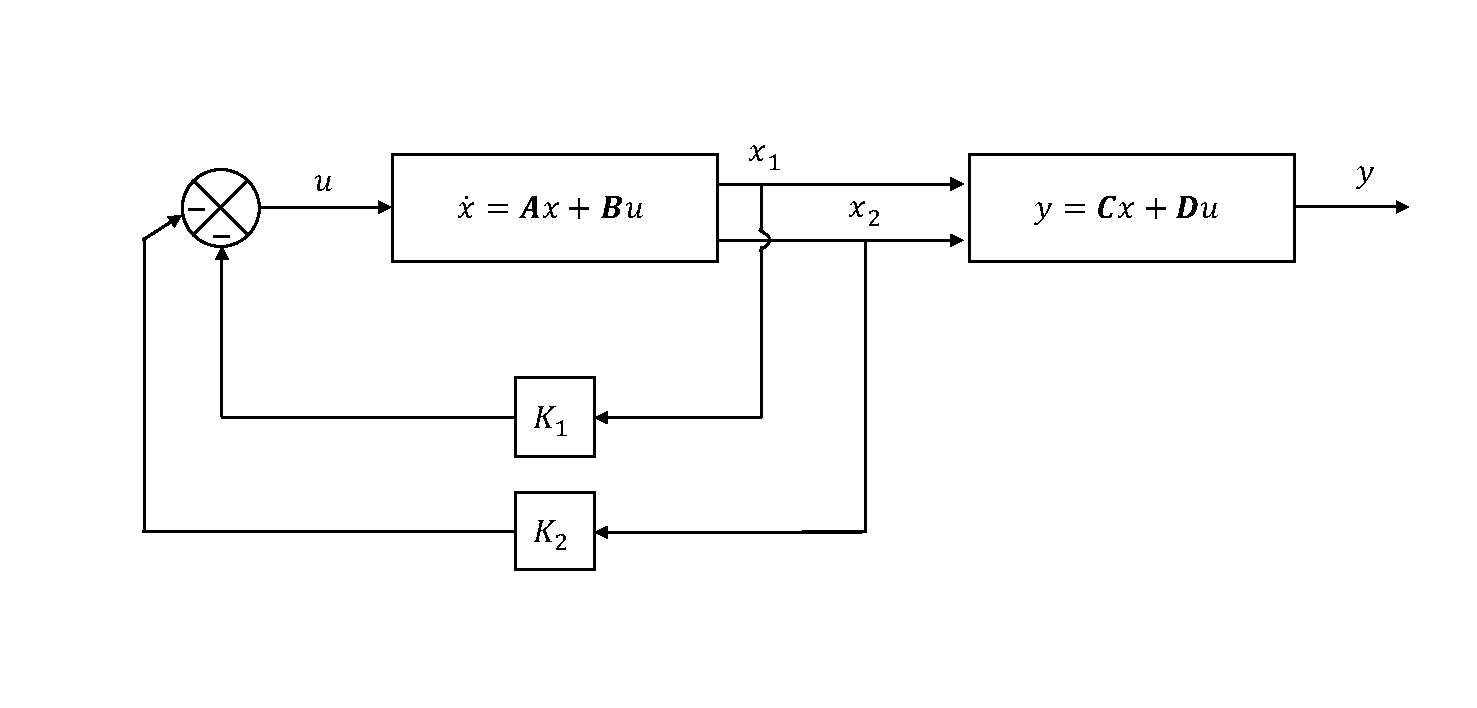
\includegraphics[scale=0.4]{diagrama.pdf}
\caption{LQR controller block diagram}
\label{fig:block_diagram}
\end{figure}

Figure \ref{fig:pendulum_control} shows simulation results with the designed LQR control system when the initial pendulum angle $\theta(0)= 5º \simeq 0.08 rad$. It can be seen how the inverted pendulum system returns to its reference position (zero).

\begin{figure}[!hbt]
\centering
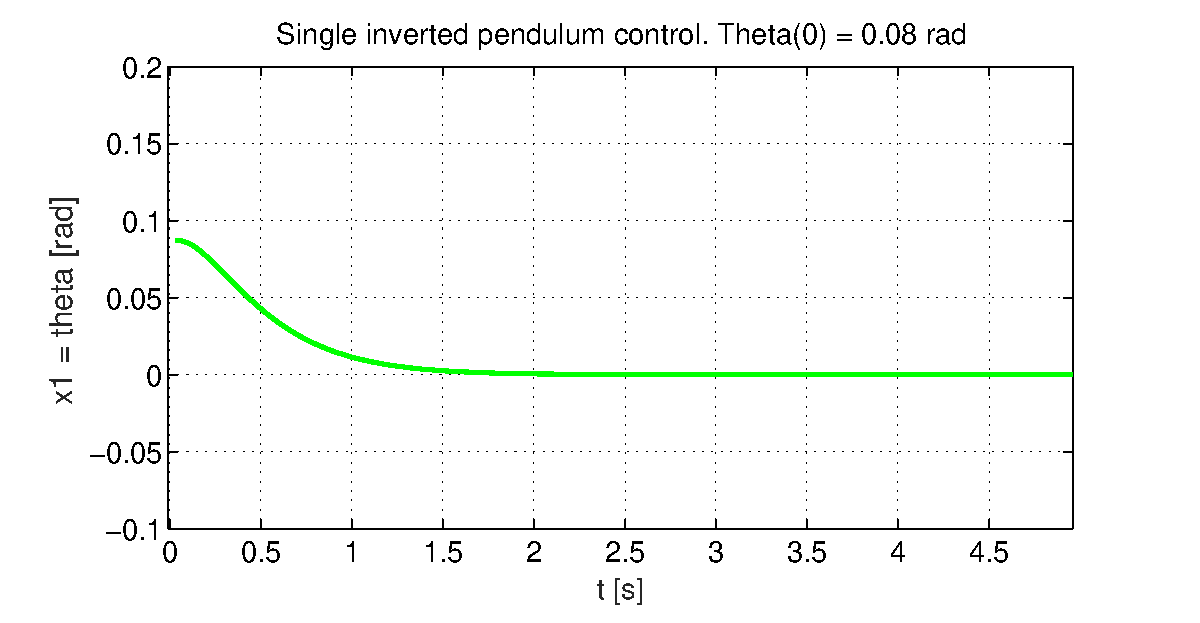
\includegraphics[scale=0.6]{00_single_inverted_pendulum_control.eps}
\caption{Linear inverted pendulum control with initial perturbations.}
\label{fig:pendulum_control}
\end{figure}

The state space representation \ref{eq:state_space}, \ref{eq:state_space_out} is a controllable canonical form that is important for the LQR controller design. It is desired to keep the actual ZMP, measured and computed by force-torque sensors located in the feet of the humanoid robot, close to its stable reference position as was discussed in previous sections. As the system is a type 0 plant, it is necessary to insert an integrator in order to design a ZMP servo control system (type 1) and remove the steady state error. Therefore, we feed the output signal $y$ (which indicates the real ZMP) back to the input and an integrator in the feedforward loop as is shown in Figure \ref{fig:diagrama_int}. Here, $z$ denotes the error between the actual and the reference ZMP, $u$ represents the commanded angle to the system and $u_D$ is the corresponding angle to the reference ZMP ($r$).

\begin{figure}[!hbt]
\centering
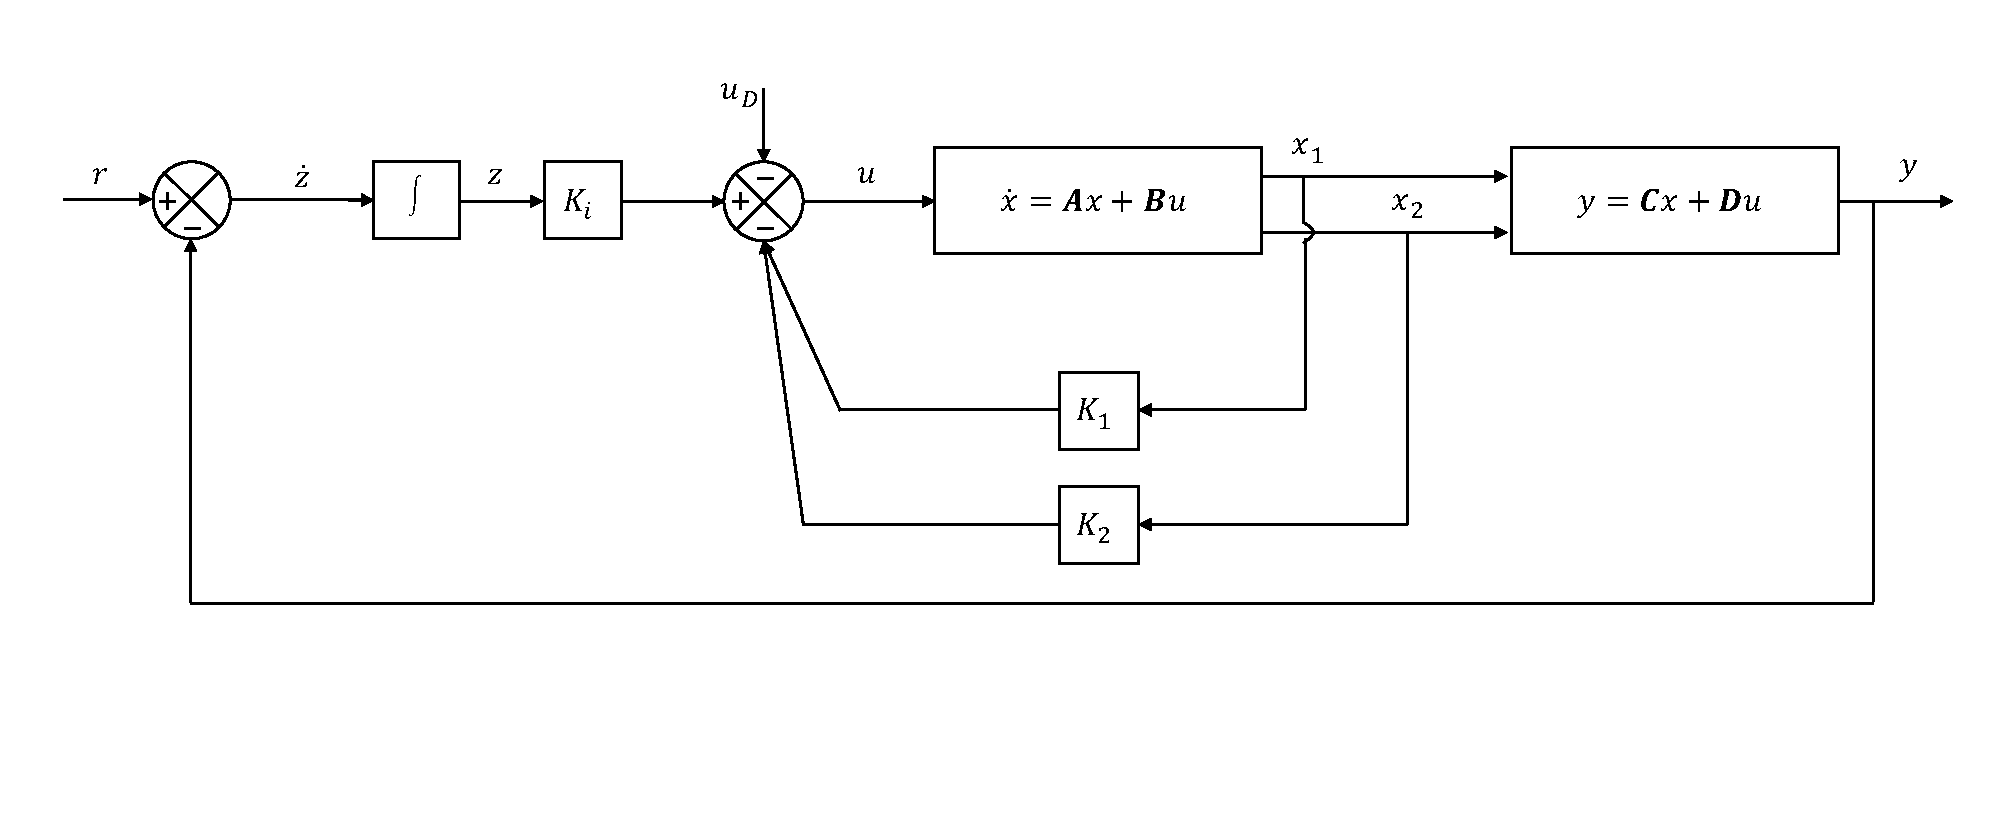
\includegraphics[scale=0.4]{diagrama_int.pdf}
\caption{ZMP LQR control system.}
\label{fig:diagrama_int}
\end{figure}

Thus, referring equations \ref{eq:state_space} and \ref{eq:state_space_out} and Figure \ref{fig:diagrama_int} and considering the actual ZMP position as the output of the system and $r$ as the reference input signal we obtain the equations for the closed loop system as follows:
\begin{equation}
\mathbf{\dot{x}} = \mathbf{A}\textbf{x} + \mathbf{B}u
\end{equation}

\begin{equation}
y = \textbf{C}\textbf{x} + \textbf{D}u
\end{equation}

\begin{equation}
u = - \textbf{K}\textbf{x} + K_i z - K_u u_D
\end{equation}

\begin{equation}
\dot{z} = r - y = r - (\textbf{C}\textbf{x} + \textbf{D}u)
\end{equation}

For the type 1 servo system, the state error equation is given by:
\begin{equation}
\begin{bmatrix}
\dot{\textbf{x}}\\
\dot{z}
\end{bmatrix} = 
\begin{bmatrix}
\textbf{A} & \textbf{0}\\
\textbf{-C} & 0
\end{bmatrix}
\begin{bmatrix}
\textbf{x}\\
z
\end{bmatrix} + 
\begin{bmatrix}
\textbf{B}\\
0
\end{bmatrix}
u
\end{equation}
and the control signal $u$ is given by:
\begin{equation}
u = \begin{bmatrix}
-\textbf{K} & K_i
\end{bmatrix}
\begin{bmatrix}
\textbf{x}\\
z 
\end{bmatrix}
- K_u u_D
\end{equation}

Figure \ref{fig:step_response} shows simulation results with the designed LQR control system with an integrator in the direct control loop. One can see how the output $y$ reaches the step reference of ZMP. Note that the output goes to negative values when the reference suddenly changes its value. This abrupt change makes the output derivative to reach higher values, so it can be solved reducing the abrupt change of the reference signal, i.e., using a ramp signal instead of a step. In Figure \ref{fig:ramp_response} the reference change is smaller and the output is smoother.

\begin{figure}[!hbt]
\centering
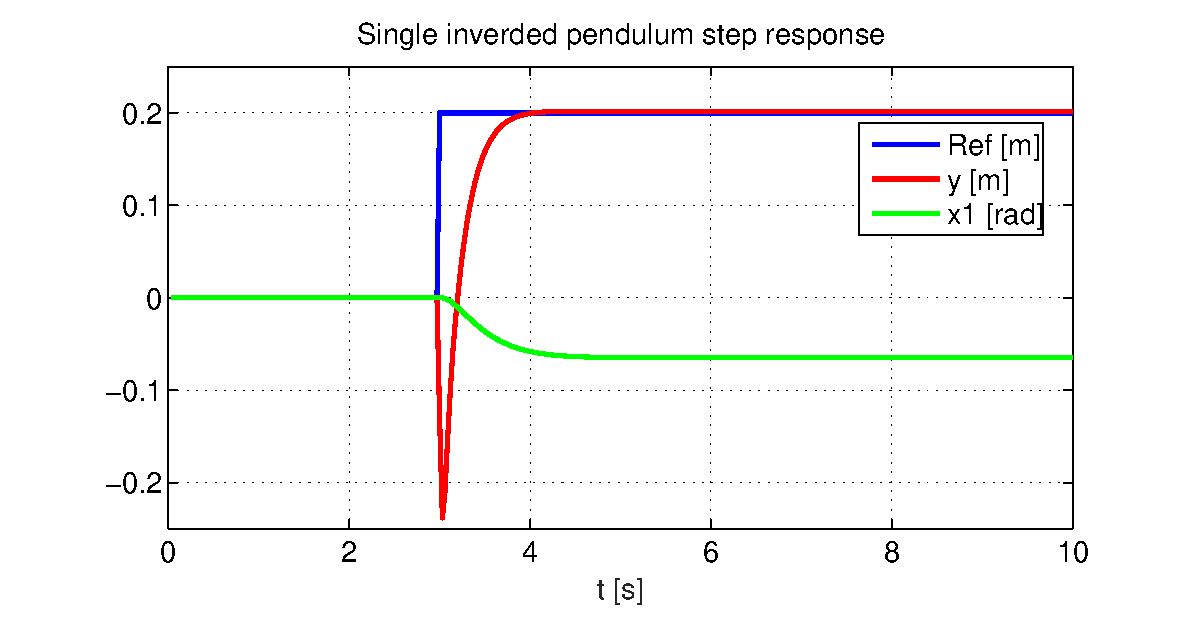
\includegraphics[scale=0.6]{010_step_response.eps}
\caption{Linear inverted pendulum step response.}
\label{fig:step_response}
\end{figure}

\begin{figure}[!hbt]
\centering
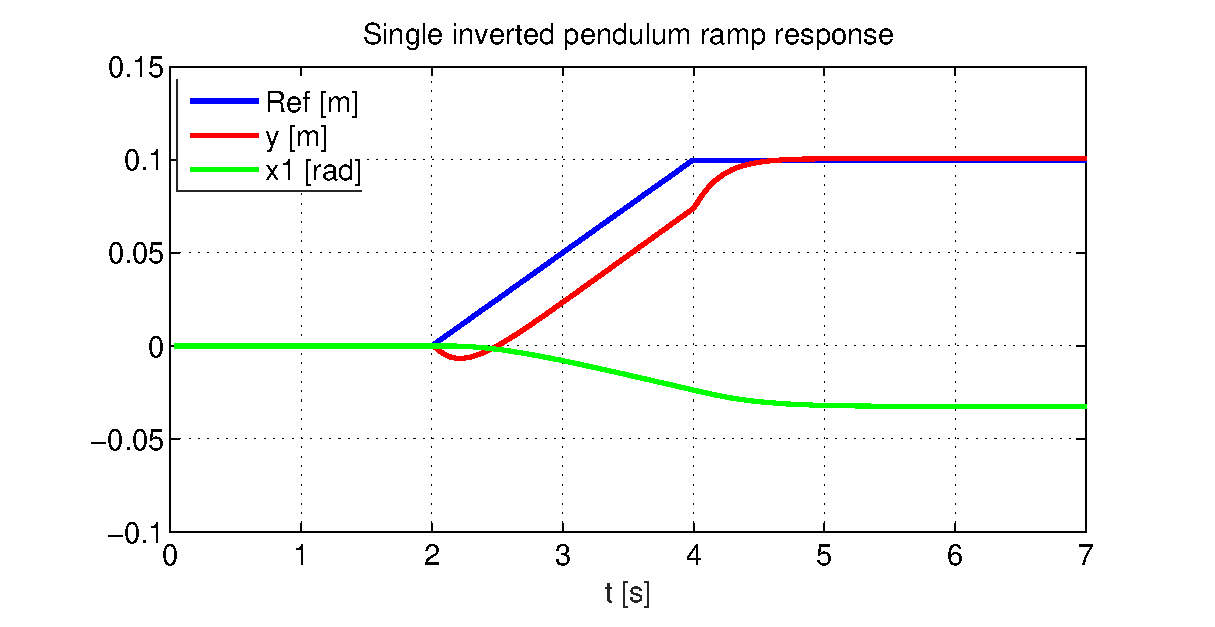
\includegraphics[scale=0.6]{011_ramp_response.eps}
\caption{Linear inverted pendulum \textcolor{red}{smooth} step response.}
\label{fig:ramp_response}
\end{figure}








